
\section*{Section A : Multiple Choice Questions [10 points] (Dan)}

\begin{enumerate}
	\item {\textbf{[2 points]} Suppose that you are using ridge regression to estimate the relationship between your data and a value of interest. Your estimate for $\hat{\beta}$ is given by:
	$$\hat{\beta} = \argmin_\beta \norm{y - X \beta}_2^2 + \lambda \norm{\beta}_2^2$$
	Where $\lambda$ is a hyper-parameter that governs how much to penalize model complexity. Which of the following would be valid ways to use a 10-fold cross validation scheme? Select all that apply.
	}
	\begin{enumerate}[label=\Alph*)]
			\item {
				 For different values of $\lambda$, train on 9 of the folds and estimate the risk on the 10th fold. Select $\lambda$ by using the value that has the lowest risk on this 10th fold. Repeat this procedure 10 times for each possible hold out and use the mean of the risks for the estimators selected at each round as an estimate of the true risk of the model.
			}
			\item {
				 For different values of $\lambda$, train on 8 of the folds and estimate the risk on the 9th fold. Select $\lambda$ by using the value that has the lowest risk on this 9th fold. Then estimate the risk using this $\lambda$ on the 10th fold. Repeat this procedure 45 (10 choose 2) times and use the mean of the risks for the estimators selected each round as an estimate of the true risk of the model.
			}
			\item {
				 For different values of $\lambda$, train on 1 of the folds, and estimate the risk on this same fold. Select $\lambda$ by using the value that has the lowest risk on this fold. Repeat this procedure 10 times (once for each fold), and use the mean of the risks for the estimators as an estimate of the true risk of the model.
			}
			\item {
				 Select a value of $\lambda$ before doing your experiment. Train on 9 of the folds and estimate the risk on the 10th fold. Repeat this procedure 10 times (once for each fold), and use the mean of the risks for the estimators as an estimate of the true risk of the model.
			}
	\end{enumerate}
	\textbf{Answer:}\underline{D}\\
	To estimate the true risk from a CV, a fix $\lambda$ should be selected first.
	
	\item {\textbf{[2 points]} For a k-Nearest Neighbor classifier and the data set below, which class will the test point (marked by the black circle) be  classified as for each of the following values of $k$? \\
	\begin{minipage}[!ht]{0.5\textwidth}
			\centering
			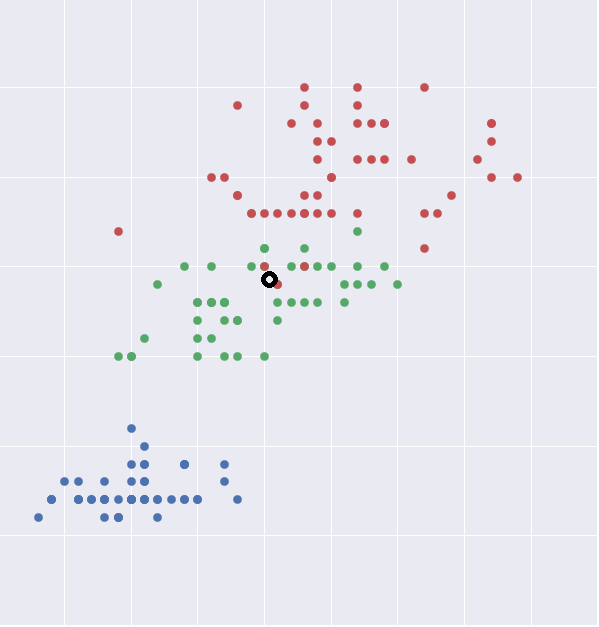
\includegraphics[width=1.0\textwidth]{knn_test_point.png}
			\label{fig:knn_test_point}
		\end{minipage}
	\begin{minipage}[!ht]{0.25\textwidth}
		\begin{enumerate}[label=(\roman*)]
			\item $k = 1$ \textbf{Answer:}\underline{A}
			\item $k = 2$ \textbf{Answer:}\underline{A}
			\item $k = 7$ \textbf{Answer:}\underline{B}
		\end{enumerate}
	\end{minipage}
	\begin{minipage}[!ht]{0.25\textwidth}
		\begin{enumerate}[label=\Alph*)]
			\item Red
			\item Green
			\item Blue
		\end{enumerate}
	\end{minipage}
	}
	
	\item {\textbf{[2 points]} Which of the following statements is true about the k-Nearest Neighbor classifier? Select all that apply.
		\begin{enumerate}[label=\Alph*)]
			\item{ As the value of $k$ increases, the variance of the model increases }
			\item{ As the value of $k$ increases, the bias of the model increases }
			\item{ As the value of $k$ increases, the model complexity increases }
			\item{ As the value of $k$ increases, the number of parameters in the model increases }
			\item{ As the number of training data points increases, the memory requirements of the model increase }
		\end{enumerate}
	}
	\textbf{Answer:}\underline{B, E}\\
	\begin{itemize}
		\item For A: the variance of the model will decrease
		\item For C: the model complexity will decrease
		\item For D: the number of parameters in the model will not change
	\end{itemize}
	
	
	\item {\textbf{[2 points]} What is the maximum training error for a decision tree on an arbitrary data set with $k$ discrete output classes?
	
		\begin{enumerate}[label=\Alph*)]
			\item $\frac{1}{k}$
			\item $1$
			\item $\frac{1}{\log_2{k}}$
			\item $\frac{k - 1}{k}$
		\end{enumerate}
	
	}
	\textbf{Answer}:\underline{D}\\
	This may happen when $P(Y)=P(Y|X_i),~\forall i$, and all data will be in a leaf node with a class label whose prior $P(Y)$ is the highest. To maximize the training error, the minimum training accuracy will be $1/k$; therefore, the maximum training error is $(k-1)/k$
	
	\item {\textbf{[2 points]} Consider the following data set. Which methods will classify all data points in this set correctly? Select all that apply. \\
		\begin{minipage}[!ht]{0.5\textwidth}
			\centering
			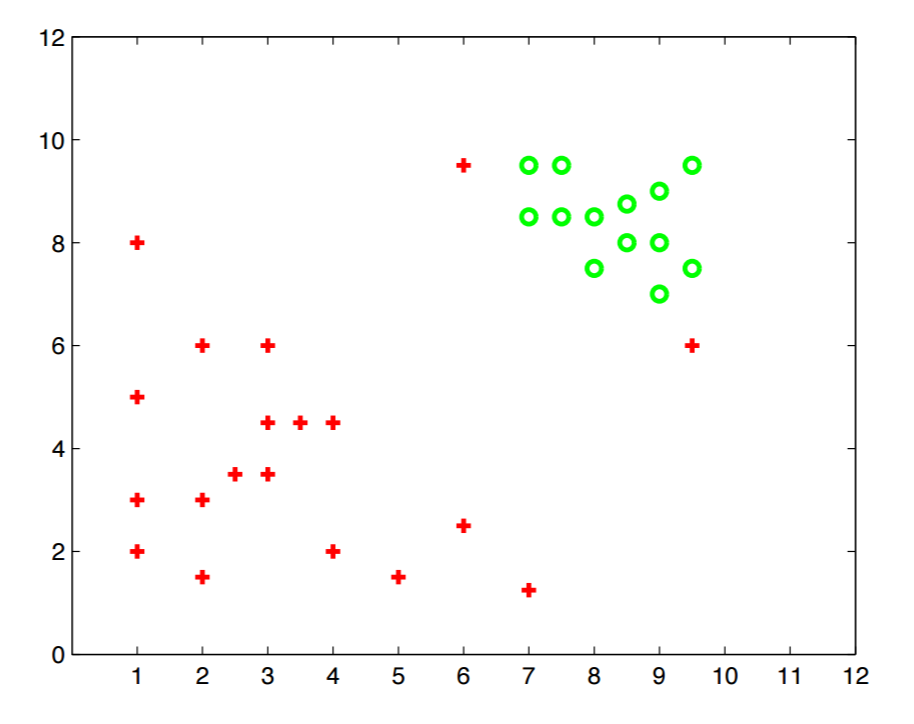
\includegraphics[width=1.0\textwidth]{mcq_data.png}
			\label{fig:svm_quad_a}
		\end{minipage}
		\begin{minipage}[!ht]{0.5\textwidth}
			\begin{enumerate}[label=\Alph*)]
				\item Soft-Margin SVM (with no kernel)
				\item SVM with a quadratic kernel, when the coefficient on the penalty for slack variables $C = 0$
				\item SVM with a quadratic kernel, when the coefficient on the penalty for slack variables $C \rightarrow \infty$
				\item Logistic regression (no kernel)
				\item 3-NN
			\end{enumerate}
		\end{minipage} 
	}
	\textbf{Answer}:\underline{C}\\
	\begin{itemize}
		\item For A: The data is not linear separable. Two outlier red points will be misclassified.
		\item For B: Because $C=0$, there will be no classification at all.
		\item For C: $C\rightarrow \infty$ means hard-margin SVM is used. The quadratic kernel is used, and the data is non-linear separable.
		\item For D: Logistic is linear classifier.
		\item For E: The two outlier red points will be misclassified.
	\end{itemize}
	
\end{enumerate}

\newpage
